\UseRawInputEncoding
\documentclass[a4paper, 14pt]{extarticle}

% Поля
%--------------------------------------
\usepackage{geometry}
\geometry{a4paper,tmargin=2cm,bmargin=2cm,lmargin=3cm,rmargin=1cm}
%--------------------------------------


%Russian-specific packages
%--------------------------------------
\usepackage[T2A]{fontenc}
\usepackage[utf8]{inputenc} 
\usepackage[english, main=russian]{babel}
\usepackage{cmap}
%--------------------------------------

\usepackage{textcomp}

% Красная строка
%--------------------------------------
\usepackage{indentfirst}               
%--------------------------------------             


%Graphics
%--------------------------------------
\usepackage{graphicx}
\graphicspath{ {./images/} }
\usepackage{wrapfig}
%--------------------------------------

% Полуторный интервал
%--------------------------------------
\linespread{1.3}                    
%--------------------------------------

%Выравнивание и переносы
%--------------------------------------
% Избавляемся от переполнений
\sloppy
% Запрещаем разрыв страницы после первой строки абзаца
\clubpenalty=10000
% Запрещаем разрыв страницы после последней строки абзаца
\widowpenalty=10000
%--------------------------------------

%Списки
\usepackage{enumitem}

%Подписи
\usepackage{caption} 

%Гиперссылки
\usepackage{hyperref}

\hypersetup {
	unicode=true
}

%Рисунки
%--------------------------------------
\DeclareCaptionLabelSeparator*{emdash}{~--- }
\captionsetup[figure]{labelsep=emdash,font=onehalfspacing,position=bottom}
%--------------------------------------

\usepackage{tempora}
\usepackage{amsmath}
\usepackage[dvipsnames]{xcolor}
\usepackage{listings}
\lstset{
  belowcaptionskip=1\baselineskip,
  breaklines=true,
  frame=L,
  xleftmargin=\parindent,
  language=Java,
  showstringspaces=false,
  basicstyle=\footnotesize\ttfamily,
  keywordstyle=\bfseries\color{blue},
  commentstyle=\itshape\color{purple},
  identifierstyle=\color{black},
  stringstyle=\color{red},
  numbers=left,           
  numberstyle=\tiny\color{gray}, 
  numbersep=10pt,      
  % ------------------------------
}

%--------------------------------------
%			НАЧАЛО ДОКУМЕНТА
%--------------------------------------

\begin{document}

%--------------------------------------
%			ТИТУЛЬНЫЙ ЛИСТ
%--------------------------------------
\begin{titlepage}
\thispagestyle{empty}
\newpage


%Шапка титульного листа
%--------------------------------------
\vspace*{-60pt}
\hspace{-65pt}
\begin{minipage}{0.3\textwidth}
\hspace*{-20pt}\centering

\includegraphics[width=\textwidth]{emblem}
\end{minipage}
\begin{minipage}{0.67\textwidth}\small \textbf{
\vspace*{-0.7ex}
\hspace*{-6pt}\centerline{Министерство науки и высшего образования Российской Федерации}
\vspace*{-0.7ex}
\centerline{Федеральное государственное бюджетное образовательное учреждение }
\vspace*{-0.7ex}
\centerline{высшего образования}
\vspace*{-0.7ex}
\centerline{<<Московский государственный технический университет}
\vspace*{-0.7ex}
\centerline{имени Н.Э. Баумана}
\vspace*{-0.7ex}
\centerline{(национальный исследовательский университет)>>}
\vspace*{-0.7ex}
\centerline{(МГТУ им. Н.Э. Баумана)}}
\end{minipage}
%--------------------------------------

%Полосы
%--------------------------------------
\vspace{-25pt}
\hspace{-35pt}\rule{\textwidth}{2.3pt}

\vspace*{-20.3pt}
\hspace{-35pt}\rule{\textwidth}{0.4pt}
%--------------------------------------

\vspace{1.5ex}
\hspace{-35pt} \noindent \small ФАКУЛЬТЕТ\hspace{80pt} <<Информатика и системы управления>>

\vspace*{-16pt}
\hspace{47pt}\rule{0.83\textwidth}{0.4pt}

\vspace{0.5ex}
\hspace{-35pt} \noindent \small КАФЕДРА\hspace{50pt} <<Теоретическая информатика и компьютерные технологии>>

\vspace*{-16pt}
\hspace{30pt}\rule{0.866\textwidth}{0.4pt}
  
\vspace{11em}

\begin{center}
\Large {\bf Летучка № 6} \\ 
\large {\bf по курсу <<Языки и методы программирования>>} \\ 
\large <<Параметризированный Stack>>
\end{center}\normalsize

\vspace{8em}


\begin{flushright}
  {Студент группы ИУ9-21Б Воронков А. С.\hspace*{15pt} \\
  \vspace{2ex}
  Преподаватель Посевин Д. П.\hspace*{15pt}}
\end{flushright}

\bigskip

\vfill
 

\begin{center}
\textsl{Москва 2026}
\end{center}
\end{titlepage}
%--------------------------------------
%		КОНЕЦ ТИТУЛЬНОГО ЛИСТА
%--------------------------------------

\renewcommand{\ttdefault}{pcr}

\setlength{\tabcolsep}{3pt}
\newpage
\setcounter{page}{2}

\section{Задание}
\begin{enumerate}
    \item Реализовать подсчет суммы следов матриц в стеке
    \item Реализовать подсчет среднего радиуса-вектора планет всех вселенных в стеке
\end{enumerate}
\section{Практическая реализация}
Код файла Stack.java
\begin{lstlisting}
import java.util.Arrays;

public class Stack<T> {
    private int count = 0;
    private Object[] buf = new Object[16];

    public boolean empty() {
        return count == 0;
    }

    public int genLen() {return count;}

    public void push(T x) {
        if (count == buf.length) {
            buf = Arrays.copyOf(buf, buf.length * 2);
        }
        buf[count++] = x;
    }
    public T check() {
        if (empty()) {
            throw new RuntimeException("underflow");
        }
        return (T)buf[count-1];
    }

    public T pop() {
        if (empty()) {
            throw new RuntimeException("underflow");
        }
        return (T)buf[--count];
    }
}
\end{lstlisting}
\par
Код файла Matrix.java
\begin{lstlisting}
public class Matrix{
    public int n;
    private int[][] mat;

    public Matrix(int n) {
        this.n = n;
        mat = new int[n][n];
    }

    public void repl(int i, int j, int x) {
        mat[i][j] = x;
    }

    public int tr() {
        int sum = 0;
        for (int i = 0; i < n; i++) {
            sum += mat[i][i];
        }
        return sum;
    }

    public String toString() {
        int mx = 0;
        for (int i = 0; i < n; i++) {
            for (int j = 0; j < n; j++) {
                mx = Math.max(mx, String.valueOf(mat[i][j]).length());
            }
        }

        StringBuilder s = new StringBuilder();
        for (int i = 0; i < n; i++) {
            s.append("[ ");
            for (int j = 0; j < n; j++) {
                s.append(String.format("%" + (mx + 1) + "d ", mat[i][j]));
            }
            s.append("]\n");
        }
        return s.toString();
    }
}
\end{lstlisting}
\par
Код файла Main1.java
\begin{lstlisting}
//TIP To <b>Run</b> code, press <shortcut actionId="Run"/> or
// click the <icon src="AllIcons.Actions.Execute"/> icon in the gutter.
public class Main1 {
    public static void main(String[] args) {
        Matrix mt1 = new Matrix(5);
        for (int i = 0; i < mt1.n; i++) {
            for (int j = 0; j < mt1.n; j++) {
                mt1.repl(i, j, i + j);
            }
        }

        int x = 0;
        Matrix mt2 = new Matrix(5);
        for (int i = 0; i < mt2.n; i++) {
            for (int j = 0; j < mt2.n; j++) {
                mt2.repl(i, j, x);
                x++;
            }
        }

        Matrix mt3 = new Matrix(4);
        for (int i = 0; i < mt3.n; i++) {
            for (int j = 0; j < mt3.n; j++) {
                mt3.repl(i, j, i - j);
            }
        }

        Stack<Matrix> s = new Stack<Matrix>();
        s.push(mt1);
        s.push(mt2);
        s.push(mt3);
        int sum = 0;
        while(!s.empty()) {
            Matrix r = s.pop();
            System.out.println(r);
            sum += r.tr();
        }
        System.out.println(sum);
    }
}
\end{lstlisting}
\par
Код файла Body.java
\begin{lstlisting}
import java.util.Date;

public class Universe {
    Stack<Body> parts;
    public Universe() {
        parts = new Stack<Body>();
    }

    public void addPart(Body... objs) {
        for (Body obj : objs) {
            parts.push(obj);
        }
    }
    public int getLen() {
        return parts.genLen();
    }
    public double[] getSumR() {
        double sumX, sumY, sumZ;
        sumX = sumY = sumZ = 0;
        Stack<Body> parts1 = new Stack<Body>();
        while (!parts.empty()) {
            Body obj = parts.pop();
            sumX += obj.getX();
            sumY += obj.getY();
            sumZ += obj.getZ();
            parts1.push(obj);
        }
        while (!parts1.empty()) {
            parts.push(parts1.pop());
        }
        return new double[]{sumX, sumY, sumZ};
    }
}
\end{lstlisting}
\par
Код файла Universe.java
\begin{lstlisting}
import java.util.Date;

public class Universe {
    Stack<Body> parts;
    public Universe() {
        parts = new Stack<Body>();
    }

    public void addPart(Body... objs) {
        for (Body obj : objs) {
            parts.push(obj);
        }
    }
    public int getLen() {
        return parts.genLen();
    }
    public double[] getSumR() {
        double sumX, sumY, sumZ;
        sumX = sumY = sumZ = 0;
        Stack<Body> parts1 = new Stack<Body>();
        while (!parts.empty()) {
            Body obj = parts.pop();
            sumX += obj.getX();
            sumY += obj.getY();
            sumZ += obj.getZ();
            parts1.push(obj);
        }
        while (!parts1.empty()) {
            parts.push(parts1.pop());
        }
        return new double[]{sumX, sumY, sumZ};
    }
}
\end{lstlisting}
\par
Код файла Main2.java
\begin{lstlisting}
import java.util.Arrays;

public class Main2 {
    public static void main(String[] args) {
        Universe universe1 = new Universe();
        for (int i = 0; i < 3; i++) {
            universe1.addPart(new Body(String.valueOf(i)));
        }
        Universe universe2 = new Universe();
        for (int i = 0; i < 4; i++) {
            universe2.addPart(new Body(String.valueOf(i)));
        }
        Universe universe3 = new Universe();
        for (int i = 0; i < 2; i++) {
            universe3.addPart(new Body(String.valueOf(i)));
        }


        Stack<Universe> s = new Stack<Universe>();
        s.push(universe1);
        s.push(universe2);
        s.push(universe3);
        double[] sum = {0, 0, 0};
        int n = 0;
        while(!s.empty()) {
            Universe u = s.pop();
            double[] r = u.getSumR();
            sum[0] += r[0];
            sum[1] += r[1];
            sum[2] += r[2];
            n+= u.getLen();
        }
        System.out.println("( " + sum[0]/n + " " + sum[1]/n + " " + sum[2]/n + " )");
    }
}
\end{lstlisting}

\begin{center}
    \nopagebreak
    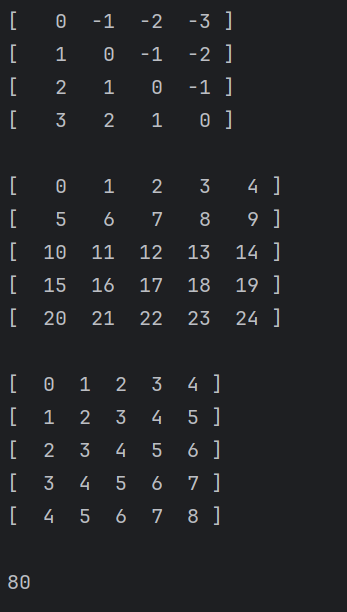
\includegraphics[width=0.85\textwidth]{let6_1}
    \captionsetup{justification=centering}
    \captionof{figure}{Результат работы Main1.java}

    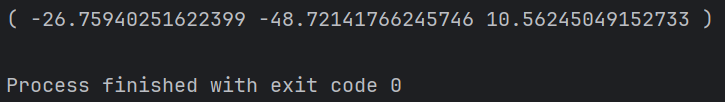
\includegraphics[width=0.85\textwidth]{let6_2}
    \captionsetup{justification=centering}
    \captionof{figure}{Результат работы Main2.java}
\end{center}

\section{Вывод}
В данной лабораторной работе были получены навыки работы с параметризированной структурой данных Stack<T>. Была написана реализация для объектов класса Matrix и Universe
\end{document}